\chapter{动态规划}

\index{动态规划}

\key{动态规划}是一种结合了
完备搜索的正确性和
贪心算法的效率的技术。
如果问题可以被分解为
可以独立求解的重叠子问题，
就可以使用动态规划。

动态规划有两种用途：

\begin{itemize}
\item
\key{寻找最优解}：
我们希望找到一个尽可能大
或尽可能小的解。
\item
\key{计算解的数量}：
我们希望计算所有
可能解的总数。
\end{itemize}

我们将首先了解如何使用动态规划
来寻找最优解，
然后再用同样的思想来
计算解的数量。

理解动态规划是每个
竞赛程序员职业生涯中的一个里程碑。
虽然基本思想很简单，
但挑战在于如何将
动态规划应用于不同的问题。
本章介绍了一组经典问题，
它们是一个很好的起点。

\section{硬币问题}

我们首先关注一个
在第6章中已经见过的问题：
给定一组硬币面值 $\texttt{coins} = \{c_1,c_2,\ldots,c_k\}$
和一个目标金额 $n$，
我们的任务是使用尽可能少的硬币
来凑成金额 $n$。

在第6章中，我们使用
贪心算法来解决这个问题，
该算法总是选择尽可能大的硬币。
例如，当硬币是欧元硬币时，
贪心算法是有效的，
但在一般情况下，贪心算法
不一定能产生最优解。

现在是时候使用动态规划
来高效地解决这个问题了，
这样算法就能适用于任何硬币集合。
动态规划算法基于一个递归函数，
该函数遍历所有凑成金额的可能方式，
就像暴力算法一样。
然而，动态规划算法是高效的，
因为它使用了\emph{记忆化}，
并且每个子问题的答案只计算一次。

\subsubsection{递归公式}

动态规划的思想是将
问题用递归的方式表达，
使得问题的解可以
从更小的子问题的解中计算出来。
在硬币问题中，一个自然的递归
问题如下：
凑成金额 $x$ 所需的最少硬币数
是多少？

令 $\texttt{solve}(x)$
表示凑成金额 $x$ 所需的
最少硬币数。
函数的值取决于
硬币的面值。
例如，如果 $\texttt{coins} = \{1,3,4\}$，
函数的前几个值如下：

\[
\begin{array}{lcl}
\texttt{solve}(0) & = & 0 \\
\texttt{solve}(1) & = & 1 \\
\texttt{solve}(2) & = & 2 \\
\texttt{solve}(3) & = & 1 \\
\texttt{solve}(4) & = & 1 \\
\texttt{solve}(5) & = & 2 \\
\texttt{solve}(6) & = & 2 \\
\texttt{solve}(7) & = & 2 \\
\texttt{solve}(8) & = & 2 \\
\texttt{solve}(9) & = & 3 \\
\texttt{solve}(10) & = & 3 \\
\end{array}
\]

例如，$\texttt{solve}(10)=3$，
因为凑成金额10至少需要3枚硬币。
最优解是 $3+3+4=10$。

$\texttt{solve}$ 的关键性质是
它的值可以
从更小的值递归地计算出来。
核心思想是关注我们为金额选择的
\emph{第一枚}硬币。
例如，在上述场景中，
第一枚硬币可以是1、3或4。
如果我们首先选择硬币1，
那么剩下的任务就是用最少的硬币
凑成金额9，
这是原问题的一个子问题。
当然，硬币3和4也是如此。
因此，我们可以使用以下递归公式
来计算最少的硬币数：
\begin{equation*}
\begin{split}
\texttt{solve}(x) = \min( & \texttt{solve}(x-1)+1, \\
                           & \texttt{solve}(x-3)+1, \\
                           & \texttt{solve}(x-4)+1).
\end{split}
\end{equation*}
递归的边界条件是 $\texttt{solve}(0)=0$，
因为凑成空金额不需要任何硬币。
例如，
\[ \texttt{solve}(10) = \texttt{solve}(7)+1 = \texttt{solve}(4)+2 = \texttt{solve}(0)+3 = 3.\]

现在我们准备给出一个通用的递归函数，
计算凑成金额 $x$ 
所需的最少硬币数：
\begin{equation*}
    \texttt{solve}(x) = \begin{cases}
               \infty               & x < 0\\
               0               & x = 0\\
               \min_{c \in \texttt{coins}} \texttt{solve}(x-c)+1 & x > 0 \\
           \end{cases}
\end{equation*}

首先，如果 $x<0$，值为 $\infty$，
因为不可能凑成负的金额。
然后，如果 $x=0$，值为 $0$，
因为凑成空金额不需要任何硬币。
最后，如果 $x>0$，变量 $c$ 遍历
选择金额的第一枚硬币的
所有可能方式。

一旦找到了解决问题的递归函数，
我们就可以直接用C++实现解决方案
（常量 \texttt{INF} 表示无穷大）：

\begin{lstlisting}
int solve(int x) {
    if (x < 0) return INF;
    if (x == 0) return 0;
    int best = INF;
    for (auto c : coins) {
        best = min(best, solve(x-c)+1);
    }
    return best;
}
\end{lstlisting}

然而，这个函数并不高效，
因为构造金额可能
有指数级数量的方式。
不过，接下来我们将看到如何使用
一种称为记忆化的技术
来使函数变得高效。

\subsubsection{使用记忆化}

\index{记忆化}

动态规划的思想是使用
\key{记忆化}来高效地计算
递归函数的值。
这意味着函数的值在计算后
会被存储在数组中。
对于每个参数，函数的值
只会递归计算一次，之后
就可以直接从数组中获取该值。

在这个问题中，我们使用数组
\begin{lstlisting}
bool ready[N];
int value[N];
\end{lstlisting}

其中 $\texttt{ready}[x]$ 表示
$\texttt{solve}(x)$ 的值是否已经被计算过，
如果是，则 $\texttt{value}[x]$
包含这个值。
常量 $N$ 的选择应确保
所有需要的值都能放入数组中。

现在这个函数可以高效地
实现如下：

\begin{lstlisting}
int solve(int x) {
    if (x < 0) return INF;
    if (x == 0) return 0;
    if (ready[x]) return value[x];
    int best = INF;
    for (auto c : coins) {
        best = min(best, solve(x-c)+1);
    }
    value[x] = best;
    ready[x] = true;
    return best;
}
\end{lstlisting}

函数像之前一样处理
边界情况 $x<0$ 和 $x=0$。
然后函数通过
$\texttt{ready}[x]$ 检查
$\texttt{solve}(x)$ 是否已经被存储
在 $\texttt{value}[x]$ 中，
如果是，函数直接返回它。
否则，函数递归地计算
$\texttt{solve}(x)$ 的值
并将其存储在 $\texttt{value}[x]$ 中。

这个函数高效地工作，
因为每个参数 $x$ 的答案
只会被递归计算一次。
在 $\texttt{solve}(x)$ 的值被存储在 $\texttt{value}[x]$ 之后，
每当函数再次以参数 $x$ 被调用时，
就可以高效地获取它。
算法的时间复杂度为 $O(nk)$，
其中 $n$ 是目标金额，$k$ 是硬币的数量。

注意，我们也可以\emph{迭代地}
构造数组 \texttt{value}，
只需使用一个循环计算
$\texttt{solve}$ 在参数 $0 \ldots n$ 上的
所有值：
\begin{lstlisting}
value[0] = 0;
for (int x = 1; x <= n; x++) {
    value[x] = INF;
    for (auto c : coins) {
        if (x-c >= 0) {
            value[x] = min(value[x], value[x-c]+1);
        }
    }
}
\end{lstlisting}

事实上，大多数竞赛程序员更喜欢这种
实现方式，因为它更短而且
常数因子更低。
从现在起，我们在示例中也
使用迭代实现。
尽管如此，用递归函数的方式来思考
动态规划解决方案通常更加容易。


\subsubsection{构造解}

有时我们不仅被要求找到
最优解的值，还被要求给出
如何构造这样一个解的示例。
例如，在硬币问题中，
我们可以声明另一个数组，
为每个金额指出
最优解中的第一枚硬币：
\begin{lstlisting}
int first[N];
\end{lstlisting}
然后，我们可以如下修改算法：
\begin{lstlisting}
value[0] = 0;
for (int x = 1; x <= n; x++) {
    value[x] = INF;
    for (auto c : coins) {
        if (x-c >= 0 && value[x-c]+1 < value[x]) {
            value[x] = value[x-c]+1;
            first[x] = c;
        }
    }
}
\end{lstlisting}
之后，可以使用以下代码
打印出金额 $n$ 的
最优解中出现的硬币：
\begin{lstlisting}
while (n > 0) {
    cout << first[n] << "\n";
    n -= first[n];
}
\end{lstlisting}

\subsubsection{计算解的数量}

现在让我们考虑硬币问题的
另一个版本，我们的任务是
计算用硬币凑成金额 $x$ 的
总方法数。
例如，如果 $\texttt{coins}=\{1,3,4\}$ 且
$x=5$，总共有6种方法：

\begin{multicols}{2}
\begin{itemize}
\item $1+1+1+1+1$
\item $1+1+3$
\item $1+3+1$
\item $3+1+1$
\item $1+4$
\item $4+1$
\end{itemize}
\end{multicols}

同样，我们可以递归地解决该问题。
令 $\texttt{solve}(x)$ 表示
我们能凑成金额 $x$ 的方法数。
例如，如果 $\texttt{coins}=\{1,3,4\}$，
那么 $\texttt{solve}(5)=6$，递归公式为
\begin{equation*}
\begin{split}
\texttt{solve}(x) = & \texttt{solve}(x-1) + \\
                    & \texttt{solve}(x-3) + \\
                    & \texttt{solve}(x-4)  .
\end{split}
\end{equation*}

然后，通用的递归函数如下：
\begin{equation*}
    \texttt{solve}(x) = \begin{cases}
               0               & x < 0\\
               1               & x = 0\\
               \sum_{c \in \texttt{coins}} \texttt{solve}(x-c) & x > 0 \\
           \end{cases}
\end{equation*}

如果 $x<0$，值为0，因为没有解。
如果 $x=0$，值为1，因为凑成空金额
只有一种方法。
否则我们计算所有形如
$\texttt{solve}(x-c)$ 的值的总和，
其中 $c$ 属于 \texttt{coins}。

以下代码构造了一个数组
$\texttt{count}$，使得
$\texttt{count}[x]$ 等于
$\texttt{solve}(x)$ 的值，
其中 $0 \le x \le n$：

\begin{lstlisting}
count[0] = 1;
for (int x = 1; x <= n; x++) {
    for (auto c : coins) {
        if (x-c >= 0) {
            count[x] += count[x-c];
        }
    }
}
\end{lstlisting}

通常解的数量非常大，
以至于不需要计算精确值，
只需给出答案模 $m$ 的结果即可，
例如 $m=10^9+7$。
这可以通过修改代码使得
所有计算都对 $m$ 取模来实现。
在上述代码中，只需在以下行之后
\begin{lstlisting}
        count[x] += count[x-c];
\end{lstlisting}
添加这一行：
\begin{lstlisting}
        count[x] %= m;
\end{lstlisting}

我们已经讨论了动态规划的
所有基本思想。
由于动态规划可以在
许多不同的情况下使用，
我们现在将通过一组问题
来进一步展示
动态规划的可能性。

\section{最长递增子序列}

\index{最长递增子序列}

我们的第一个问题是
在包含 $n$ 个元素的数组中找到
\key{最长递增子序列}。
这是一个从左到右的、最大长度的
数组元素序列，
且序列中的每个元素都大于
前一个元素。
例如，在数组

\begin{center}
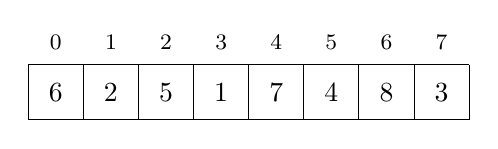
\begin{tikzpicture}[scale=0.7]
\draw (0,0) grid (8,1);
\node at (0.5,0.5) {$6$};
\node at (1.5,0.5) {$2$};
\node at (2.5,0.5) {$5$};
\node at (3.5,0.5) {$1$};
\node at (4.5,0.5) {$7$};
\node at (5.5,0.5) {$4$};
\node at (6.5,0.5) {$8$};
\node at (7.5,0.5) {$3$};

\footnotesize
\node at (0.5,1.4) {$0$};
\node at (1.5,1.4) {$1$};
\node at (2.5,1.4) {$2$};
\node at (3.5,1.4) {$3$};
\node at (4.5,1.4) {$4$};
\node at (5.5,1.4) {$5$};
\node at (6.5,1.4) {$6$};
\node at (7.5,1.4) {$7$};
\end{tikzpicture}
\end{center}
最长递增子序列
包含4个元素：
\begin{center}
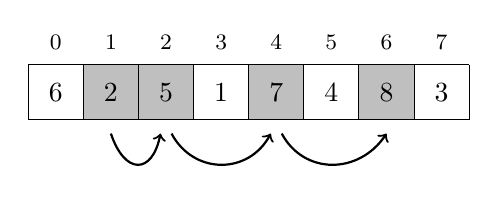
\begin{tikzpicture}[scale=0.7]
\fill[color=lightgray] (1,0) rectangle (2,1);
\fill[color=lightgray] (2,0) rectangle (3,1);
\fill[color=lightgray] (4,0) rectangle (5,1);
\fill[color=lightgray] (6,0) rectangle (7,1);
\draw (0,0) grid (8,1);
\node at (0.5,0.5) {$6$};
\node at (1.5,0.5) {$2$};
\node at (2.5,0.5) {$5$};
\node at (3.5,0.5) {$1$};
\node at (4.5,0.5) {$7$};
\node at (5.5,0.5) {$4$};
\node at (6.5,0.5) {$8$};
\node at (7.5,0.5) {$3$};

\draw[thick,->] (1.5,-0.25) .. controls (1.75,-1.00) and (2.25,-1.00) .. (2.4,-0.25);
\draw[thick,->] (2.6,-0.25) .. controls (3.0,-1.00) and (4.0,-1.00) .. (4.4,-0.25);
\draw[thick,->] (4.6,-0.25) .. controls (5.0,-1.00) and (6.0,-1.00) .. (6.5,-0.25);

\footnotesize
\node at (0.5,1.4) {$0$};
\node at (1.5,1.4) {$1$};
\node at (2.5,1.4) {$2$};
\node at (3.5,1.4) {$3$};
\node at (4.5,1.4) {$4$};
\node at (5.5,1.4) {$5$};
\node at (6.5,1.4) {$6$};
\node at (7.5,1.4) {$7$};
\end{tikzpicture}
\end{center}

令 $\texttt{length}(k)$ 表示
以位置 $k$ 结尾的
最长递增子序列的长度。
因此，如果我们计算
$\texttt{length}(k)$ 在 $0 \le k \le n-1$ 范围内的所有值，
我们就能找到
最长递增子序列的长度。
例如，上述数组对应的
函数值如下：
\[
\begin{array}{lcl}
\texttt{length}(0) & = & 1 \\
\texttt{length}(1) & = & 1 \\
\texttt{length}(2) & = & 2 \\
\texttt{length}(3) & = & 1 \\
\texttt{length}(4) & = & 3 \\
\texttt{length}(5) & = & 2 \\
\texttt{length}(6) & = & 4 \\
\texttt{length}(7) & = & 2 \\
\end{array}
\]

例如，$\texttt{length}(6)=4$，
因为以位置6结尾的最长递增子序列
由4个元素组成。

为了计算 $\texttt{length}(k)$ 的值，
我们需要找到一个位置 $i<k$，
使得 $\texttt{array}[i]<\texttt{array}[k]$
且 $\texttt{length}(i)$ 尽可能大。
然后我们知道
$\texttt{length}(k)=\texttt{length}(i)+1$，
因为这是将 $\texttt{array}[k]$ 
添加到子序列中的最优方式。
然而，如果不存在这样的位置 $i$，
则 $\texttt{length}(k)=1$，
这意味着子序列仅包含
$\texttt{array}[k]$。

由于函数的所有值都可以
从更小的值计算出来，
我们可以使用动态规划。
在以下代码中，函数的值
将被存储在数组
$\texttt{length}$ 中。

\begin{lstlisting}
for (int k = 0; k < n; k++) {
    length[k] = 1;
    for (int i = 0; i < k; i++) {
        if (array[i] < array[k]) {
            length[k] = max(length[k],length[i]+1);
        }
    }
}
\end{lstlisting}

这段代码的时间复杂度为 $O(n^2)$，
因为它由两层嵌套循环组成。
然而，也可以用 $O(n \log n)$ 的时间
更高效地实现
动态规划计算。
你能找到实现方法吗？

\section{网格中的路径}

我们的下一个问题是
在 $n \times n$ 网格中找到一条
从左上角到
右下角的路径，
使得我们只向下和向右移动。
每个格子包含一个正整数，
路径的构造应使
沿路径的值之和尽可能大。

下图展示了一个网格中的
最优路径：
\begin{center}
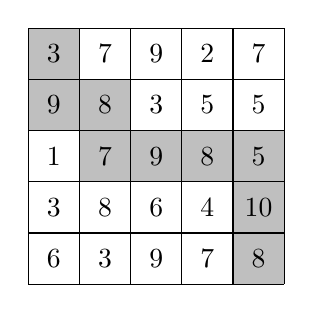
\begin{tikzpicture}[scale=.65]
  \begin{scope}
    \fill [color=lightgray] (0, 9) rectangle (1, 8);
    \fill [color=lightgray] (0, 8) rectangle (1, 7);
    \fill [color=lightgray] (1, 8) rectangle (2, 7);
    \fill [color=lightgray] (1, 7) rectangle (2, 6);
    \fill [color=lightgray] (2, 7) rectangle (3, 6);
    \fill [color=lightgray] (3, 7) rectangle (4, 6);
    \fill [color=lightgray] (4, 7) rectangle (5, 6);
    \fill [color=lightgray] (4, 6) rectangle (5, 5);
    \fill [color=lightgray] (4, 5) rectangle (5, 4);
    \draw (0, 4) grid (5, 9);
    \node at (0.5,8.5) {3};
    \node at (1.5,8.5) {7};
    \node at (2.5,8.5) {9};
    \node at (3.5,8.5) {2};
    \node at (4.5,8.5) {7};
    \node at (0.5,7.5) {9};
    \node at (1.5,7.5) {8};
    \node at (2.5,7.5) {3};
    \node at (3.5,7.5) {5};
    \node at (4.5,7.5) {5};
    \node at (0.5,6.5) {1};
    \node at (1.5,6.5) {7};
    \node at (2.5,6.5) {9};
    \node at (3.5,6.5) {8};
    \node at (4.5,6.5) {5};
    \node at (0.5,5.5) {3};
    \node at (1.5,5.5) {8};
    \node at (2.5,5.5) {6};
    \node at (3.5,5.5) {4};
    \node at (4.5,5.5) {10};
    \node at (0.5,4.5) {6};
    \node at (1.5,4.5) {3};
    \node at (2.5,4.5) {9};
    \node at (3.5,4.5) {7};
    \node at (4.5,4.5) {8};
  \end{scope}
\end{tikzpicture}
\end{center}
路径上值之和为67，
这是从
左上角到右下角的路径上
可能的最大和。

假设网格的行和列
从1到 $n$ 编号，
且 $\texttt{value}[y][x]$ 等于
格子 $(y,x)$ 的值。
令 $\texttt{sum}(y,x)$ 表示
从左上角到格子 $(y,x)$ 的
路径上的最大和。
现在 $\texttt{sum}(n,n)$ 告诉我们
从左上角到
右下角的最大和。
例如，在上述网格中，
$\texttt{sum}(5,5)=67$。

我们可以递归地计算
这些和如下：
\[ \texttt{sum}(y,x) = \max(\texttt{sum}(y,x-1),\texttt{sum}(y-1,x))+\texttt{value}[y][x]\]


递归公式基于这样的观察：
到达格子 $(y,x)$ 的路径
要么来自格子 $(y,x-1)$，
要么来自格子 $(y-1,x)$：
\begin{center}
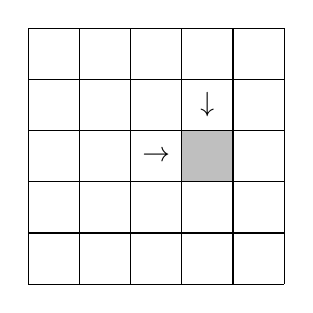
\begin{tikzpicture}[scale=.65]
  \begin{scope}
    \fill [color=lightgray] (3, 7) rectangle (4, 6);
    \draw (0, 4) grid (5, 9);
    
    \node at (2.5,6.5) {$\rightarrow$};
    \node at (3.5,7.5) {$\downarrow$};
    
  \end{scope}
\end{tikzpicture}
\end{center}

因此，我们选择使和
最大化的方向。
我们假设当 $y=0$ 或 $x=0$ 时
$\texttt{sum}(y,x)=0$
（因为这样的路径不存在），
所以递归公式在 $y=1$ 或 $x=1$ 时也适用。

由于函数 \texttt{sum} 有两个参数，
动态规划数组也有两个维度。
例如，我们可以使用数组
\begin{lstlisting}
int sum[N][N];
\end{lstlisting}
并按如下方式计算和：
\begin{lstlisting}
for (int y = 1; y <= n; y++) {
    for (int x = 1; x <= n; x++) {
        sum[y][x] = max(sum[y][x-1],sum[y-1][x])+value[y][x];
    }
}
\end{lstlisting}
算法的时间复杂度为 $O(n^2)$。

\section{背包问题}

\index{背包}

术语\key{背包}指的是这样一类问题：
给定一组物品，
需要找出
具有某些性质的子集。
背包问题通常可以使用
动态规划来解决。

在本节中，我们关注以下问题：
给定一个权重列表
$[w_1,w_2,\ldots,w_n]$，
确定可以使用这些权重
构造的所有和。
例如，如果权重为
$[1,3,3,5]$，以下和是可能的：

\begin{center}
\begin{tabular}{rrrrrrrrrrrrr}
 0 & 1 & 2 & 3 & 4 & 5 & 6 & 7 & 8 & 9 & 10 & 11 & 12 \\
\hline
 X & X & & X & X & X & X & X & X & X & & X & X \\
\end{tabular}
\end{center}

在这种情况下，$0 \ldots 12$ 之间的所有和
都是可能的，除了2和10。
例如，和7是可能的，因为我们
可以选择权重 $[1,3,3]$。

为了解决这个问题，我们关注子问题，
即仅使用前 $k$ 个权重
来构造和。
令 $\texttt{possible}(x,k)=\textrm{true}$ 表示
我们可以用前 $k$ 个权重
构造和 $x$，
否则 $\texttt{possible}(x,k)=\textrm{false}$。
函数的值可以
递归地计算如下：
\[ \texttt{possible}(x,k) = \texttt{possible}(x-w_k,k-1) \lor \texttt{possible}(x,k-1) \]
该公式基于这样一个事实：
我们可以选择使用或不使用
权重 $w_k$ 来构造和。
如果使用 $w_k$，剩余的任务是
用前 $k-1$ 个权重凑成和 $x-w_k$，
如果不使用 $w_k$，
剩余的任务是用前 $k-1$ 个权重
凑成和 $x$。
作为边界条件，
\begin{equation*}
    \texttt{possible}(x,0) = \begin{cases}
               \textrm{true}    & x = 0\\
               \textrm{false}   & x \neq 0 \\
           \end{cases}
\end{equation*}
因为如果不使用任何权重，
我们只能凑成和0。

下表展示了权重 $[1,3,3,5]$ 的
所有函数值（符号''X''
表示真值）：

\begin{center}
\begin{tabular}{r|rrrrrrrrrrrrr}
$k \backslash x$ & 0 & 1 & 2 & 3 & 4 & 5 & 6 & 7 & 8 & 9 & 10 & 11 & 12 \\
\hline
 0 & X & \\
 1 & X & X \\
 2 & X & X & & X & X \\
 3 & X & X & & X & X & & X & X \\
 4 & X & X & & X & X & X & X & X & X & X & & X & X \\
\end{tabular}
\end{center}

计算完这些值后，$\texttt{possible}(x,n)$
告诉我们是否可以使用\emph{所有}权重
构造和 $x$。

令 $W$ 表示权重的总和。
以下 $O(nW)$ 时间的
动态规划解决方案
对应于该递归函数：
\begin{lstlisting}
possible[0][0] = true;
for (int k = 1; k <= n; k++) {
    for (int x = 0; x <= W; x++) {
        if (x-w[k] >= 0) possible[x][k] |= possible[x-w[k]][k-1];
        possible[x][k] |= possible[x][k-1];
    }
}
\end{lstlisting}

然而，这里有一个更好的实现，
只使用一维数组 $\texttt{possible}[x]$，
该数组指示我们是否能构造一个和为 $x$ 的子集。
技巧是对于每个新权重，
从右到左更新数组：
\begin{lstlisting}
possible[0] = true;
for (int k = 1; k <= n; k++) {
    for (int x = W; x >= 0; x--) {
        if (possible[x]) possible[x+w[k]] = true;
    }
}
\end{lstlisting}

注意，这里介绍的一般思想可以用于
许多背包问题。
例如，如果给定具有权重和价值的物品，
我们可以确定每个权重和对应的子集的
最大价值和。

\section{编辑距离}

\index{编辑距离}
\index{Levenshtein距离}

\key{编辑距离}或\key{Levenshtein距离}\footnote{该距离
以V. I. Levenshtein的名字命名，他在研究二进制码时研究了这一概念 \cite{lev66}。}
是将一个字符串
变换为另一个字符串所需的
最少编辑操作数。
允许的编辑操作如下：
\begin{itemize}
\item 插入一个字符（例如 \texttt{ABC} $\rightarrow$ \texttt{ABCA}）
\item 删除一个字符（例如 \texttt{ABC} $\rightarrow$ \texttt{AC}）
\item 修改一个字符（例如 \texttt{ABC} $\rightarrow$ \texttt{ADC}）
\end{itemize}

例如，\texttt{LOVE} 和 \texttt{MOVIE} 之间的编辑距离为2，
因为我们可以首先执行操作
 \texttt{LOVE} $\rightarrow$ \texttt{MOVE}
（修改），然后执行操作
\texttt{MOVE} $\rightarrow$ \texttt{MOVIE}
（插入）。
这是可能的最少操作数，
因为显然仅用一次操作是不够的。

假设给定长度为 $n$ 的字符串 \texttt{x}
和长度为 $m$ 的字符串 \texttt{y}，
我们想计算
\texttt{x} 和 \texttt{y} 之间的编辑距离。
为了解决这个问题，我们定义一个函数
$\texttt{distance}(a,b)$，
它给出前缀
$\texttt{x}[0 \ldots a]$ 和 $\texttt{y}[0 \ldots b]$ 之间的
编辑距离。
因此，使用这个函数，
\texttt{x} 和 \texttt{y} 之间的编辑距离等于 $\texttt{distance}(n-1,m-1)$。

我们可以如下计算 \texttt{distance} 的值：
\begin{equation*}
\begin{split}
\texttt{distance}(a,b) = \min(& \texttt{distance}(a,b-1)+1, \\
                           & \texttt{distance}(a-1,b)+1, \\
                           & \texttt{distance}(a-1,b-1)+\texttt{cost}(a,b)).
\end{split}
\end{equation*}
这里如果 $\texttt{x}[a]=\texttt{y}[b]$ 则 $\texttt{cost}(a,b)=0$，
否则 $\texttt{cost}(a,b)=1$。
该公式考虑了以下编辑
字符串 \texttt{x} 的方式：
\begin{itemize}
\item $\texttt{distance}(a,b-1)$：在 \texttt{x} 的末尾插入一个字符
\item $\texttt{distance}(a-1,b)$：删除 \texttt{x} 的最后一个字符
\item $\texttt{distance}(a-1,b-1)$：匹配或修改 \texttt{x} 的最后一个字符
\end{itemize}
在前两种情况下，需要一次编辑操作
（插入或删除）。
在最后一种情况下，如果 $\texttt{x}[a]=\texttt{y}[b]$，
我们可以匹配最后一个字符而无需编辑，
否则需要一次编辑操作（修改）。

下表展示了示例情况中
\texttt{distance} 的值：
\begin{center}
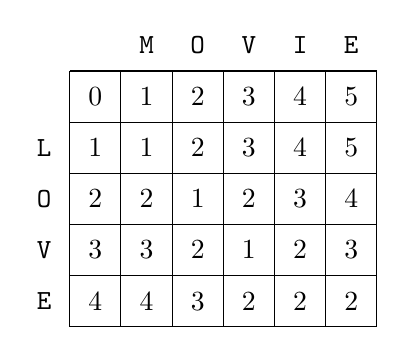
\begin{tikzpicture}[scale=.65]
  \begin{scope}
    %\fill [color=lightgray] (5, -3) rectangle (6, -4);
    \draw (1, -1) grid (7, -6);
    
    \node at (0.5,-2.5) {\texttt{L}};
    \node at (0.5,-3.5) {\texttt{O}};
    \node at (0.5,-4.5) {\texttt{V}};
    \node at (0.5,-5.5) {\texttt{E}};

    \node at (2.5,-0.5) {\texttt{M}};
    \node at (3.5,-0.5) {\texttt{O}};
    \node at (4.5,-0.5) {\texttt{V}};
    \node at (5.5,-0.5) {\texttt{I}};
    \node at (6.5,-0.5) {\texttt{E}};

    \node at (1.5,-1.5) {$0$};
    \node at (1.5,-2.5) {$1$};
    \node at (1.5,-3.5) {$2$};
    \node at (1.5,-4.5) {$3$};
    \node at (1.5,-5.5) {$4$};
    \node at (2.5,-1.5) {$1$};
    \node at (2.5,-2.5) {$1$};
    \node at (2.5,-3.5) {$2$};
    \node at (2.5,-4.5) {$3$};
    \node at (2.5,-5.5) {$4$};
    \node at (3.5,-1.5) {$2$};
    \node at (3.5,-2.5) {$2$};
    \node at (3.5,-3.5) {$1$};
    \node at (3.5,-4.5) {$2$};
    \node at (3.5,-5.5) {$3$};
    \node at (4.5,-1.5) {$3$};
    \node at (4.5,-2.5) {$3$};
    \node at (4.5,-3.5) {$2$};
    \node at (4.5,-4.5) {$1$};
    \node at (4.5,-5.5) {$2$};
    \node at (5.5,-1.5) {$4$};
    \node at (5.5,-2.5) {$4$};
    \node at (5.5,-3.5) {$3$};
    \node at (5.5,-4.5) {$2$};
    \node at (5.5,-5.5) {$2$};
    \node at (6.5,-1.5) {$5$};
    \node at (6.5,-2.5) {$5$};
    \node at (6.5,-3.5) {$4$};
    \node at (6.5,-4.5) {$3$};
    \node at (6.5,-5.5) {$2$};
  \end{scope}
\end{tikzpicture}
\end{center}

表格的右下角
告诉我们 \texttt{LOVE} 和 \texttt{MOVIE} 
之间的编辑距离为2。
表格还展示了如何构造
最短的编辑操作序列。
在这种情况下，路径如下：

\begin{center}
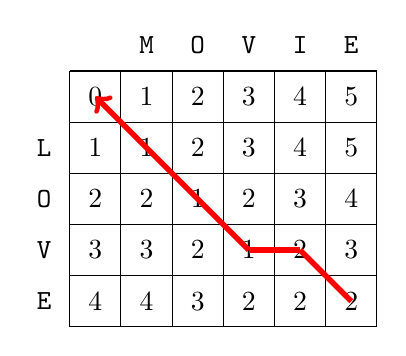
\begin{tikzpicture}[scale=.65]
  \begin{scope}
    \draw (1, -1) grid (7, -6);
    
    \node at (0.5,-2.5) {\texttt{L}};
    \node at (0.5,-3.5) {\texttt{O}};
    \node at (0.5,-4.5) {\texttt{V}};
    \node at (0.5,-5.5) {\texttt{E}};

    \node at (2.5,-0.5) {\texttt{M}};
    \node at (3.5,-0.5) {\texttt{O}};
    \node at (4.5,-0.5) {\texttt{V}};
    \node at (5.5,-0.5) {\texttt{I}};
    \node at (6.5,-0.5) {\texttt{E}};

    \node at (1.5,-1.5) {$0$};
    \node at (1.5,-2.5) {$1$};
    \node at (1.5,-3.5) {$2$};
    \node at (1.5,-4.5) {$3$};
    \node at (1.5,-5.5) {$4$};
    \node at (2.5,-1.5) {$1$};
    \node at (2.5,-2.5) {$1$};
    \node at (2.5,-3.5) {$2$};
    \node at (2.5,-4.5) {$3$};
    \node at (2.5,-5.5) {$4$};
    \node at (3.5,-1.5) {$2$};
    \node at (3.5,-2.5) {$2$};
    \node at (3.5,-3.5) {$1$};
    \node at (3.5,-4.5) {$2$};
    \node at (3.5,-5.5) {$3$};
    \node at (4.5,-1.5) {$3$};
    \node at (4.5,-2.5) {$3$};
    \node at (4.5,-3.5) {$2$};
    \node at (4.5,-4.5) {$1$};
    \node at (4.5,-5.5) {$2$};
    \node at (5.5,-1.5) {$4$};
    \node at (5.5,-2.5) {$4$};
    \node at (5.5,-3.5) {$3$};
    \node at (5.5,-4.5) {$2$};
    \node at (5.5,-5.5) {$2$};
    \node at (6.5,-1.5) {$5$};
    \node at (6.5,-2.5) {$5$};
    \node at (6.5,-3.5) {$4$};
    \node at (6.5,-4.5) {$3$};
    \node at (6.5,-5.5) {$2$};

    \path[draw=red,thick,-,line width=2pt] (6.5,-5.5) -- (5.5,-4.5);
    \path[draw=red,thick,-,line width=2pt] (5.5,-4.5) -- (4.5,-4.5);
    \path[draw=red,thick,->,line width=2pt] (4.5,-4.5) -- (1.5,-1.5);
  \end{scope}
\end{tikzpicture}
\end{center}

\texttt{LOVE} 和 \texttt{MOVIE} 的最后一个字符
相同，因此它们之间的编辑距离
等于 \texttt{LOV} 和 \texttt{MOVI} 之间的编辑距离。
我们可以用一次编辑操作从
\texttt{MOVI} 中删除字符 \texttt{I}。
因此，编辑距离比
\texttt{LOV} 和 \texttt{MOV} 之间的编辑距离大1，以此类推。

\section{计算铺方案}

有时动态规划解的状态
比数字的固定组合更加复杂。
作为一个例子，
考虑计算使用
$1 \times 2$ 和 $2 \times 1$ 大小的瓷砖
填充 $n \times m$ 网格的
不同方法数。
例如，$4 \times 7$ 网格的一个有效解是
\begin{center}
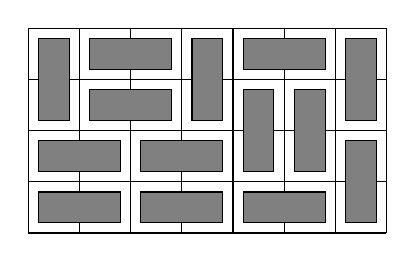
\begin{tikzpicture}[scale=.65]
    \draw (0,0) grid (7,4);
    \draw[fill=gray] (0+0.2,0+0.2) rectangle (2-0.2,1-0.2);
    \draw[fill=gray] (2+0.2,0+0.2) rectangle (4-0.2,1-0.2);
    \draw[fill=gray] (4+0.2,0+0.2) rectangle (6-0.2,1-0.2);
    \draw[fill=gray] (0+0.2,1+0.2) rectangle (2-0.2,2-0.2);
    \draw[fill=gray] (2+0.2,1+0.2) rectangle (4-0.2,2-0.2);
    \draw[fill=gray] (1+0.2,2+0.2) rectangle (3-0.2,3-0.2);
    \draw[fill=gray] (1+0.2,3+0.2) rectangle (3-0.2,4-0.2);
    \draw[fill=gray] (4+0.2,3+0.2) rectangle (6-0.2,4-0.2);

    \draw[fill=gray] (0+0.2,2+0.2) rectangle (1-0.2,4-0.2);
    \draw[fill=gray] (3+0.2,2+0.2) rectangle (4-0.2,4-0.2);
    \draw[fill=gray] (6+0.2,2+0.2) rectangle (7-0.2,4-0.2);
    \draw[fill=gray] (4+0.2,1+0.2) rectangle (5-0.2,3-0.2);
    \draw[fill=gray] (5+0.2,1+0.2) rectangle (6-0.2,3-0.2);
    \draw[fill=gray] (6+0.2,0+0.2) rectangle (7-0.2,2-0.2);

\end{tikzpicture}
\end{center}
总解数为781。

这个问题可以用动态规划解决，
方法是逐行遍历网格。
解中的每一行可以表示为
一个包含 $m$ 个字符的字符串，
字符取自集合
$\{\sqcap, \sqcup, \sqsubset, \sqsupset \}$。
例如，上述解由四行组成，
对应以下字符串：
\begin{itemize}
\item
$\sqcap \sqsubset \sqsupset \sqcap \sqsubset \sqsupset \sqcap$
\item
$\sqcup \sqsubset \sqsupset \sqcup \sqcap \sqcap \sqcup$
\item
$\sqsubset \sqsupset \sqsubset \sqsupset \sqcup \sqcup \sqcap$ 
\item
$\sqsubset \sqsupset \sqsubset \sqsupset \sqsubset \sqsupset \sqcup$
\end{itemize}

令 $\texttt{count}(k,x)$ 表示
为网格的第 $1 \ldots k$ 行
构造解的方法数，
其中字符串 $x$ 对应第 $k$ 行。
这里可以使用动态规划，
因为一行的状态仅受
前一行的状态约束。

一个解是有效的当且仅当第1行不包含
字符 $\sqcup$，
第 $n$ 行不包含字符 $\sqcap$，
且所有相邻行都是\emph{兼容的}。
例如，行
$\sqcup \sqsubset \sqsupset \sqcup \sqcap \sqcap \sqcup$ 和
$\sqsubset \sqsupset \sqsubset \sqsupset \sqcup \sqcup \sqcap$ 
是兼容的，而行
$\sqcap \sqsubset \sqsupset \sqcap \sqsubset \sqsupset \sqcap$ 和
$\sqsubset \sqsupset \sqsubset \sqsupset \sqsubset \sqsupset \sqcup$
是不兼容的。

由于一行由 $m$ 个字符组成，
每个字符有四种选择，
因此不同行的数量最多为 $4^m$。
因此，解决方案的时间复杂度为
$O(n 4^{2m})$，因为对于每一行，
我们需要遍历 $O(4^m)$ 个可能状态，
而对于每个状态，前一行的
可能状态有 $O(4^m)$ 个。
实际上，旋转网格使得
较短边的长度为 $m$ 是一个好主意，
因为因子 $4^{2m}$ 主导了时间复杂度。

通过使用更紧凑的行表示方法，
可以使解决方案更加高效。
事实上，只需要知道前一行的哪些列
包含竖直瓷砖的上半部分就足够了。
因此，我们可以仅使用字符
$\sqcap$ 和 $\Box$ 来表示一行，
其中 $\Box$ 是字符
$\sqcup$、$\sqsubset$ 和 $\sqsupset$ 的组合。
使用这种表示方法，
仅有 $2^m$ 种不同的行，
时间复杂度为 $O(n 2^{2m})$。

最后值得一提的是，还有一个令人惊讶的直接公式
用于计算铺方案数\footnote{令人惊讶的是，
这个公式是在1961年由两个研究团队 \cite{kas61,tem61}
独立发现的。}：
\[ \prod_{a=1}^{\lceil n/2 \rceil} \prod_{b=1}^{\lceil m/2 \rceil} 4 \cdot (\cos^2 \frac{\pi a}{n + 1} + \cos^2 \frac{\pi b}{m+1})\]
这个公式非常高效，因为它可以在 $O(nm)$ 时间内
计算出铺方案数，
但由于答案是实数的乘积，
使用该公式时的一个问题是
如何准确地存储中间结果。


